\RequirePackage{luatex85}
\documentclass{standalone}

\usepackage{fontspec}
\usepackage{bm}
\usepackage{commath}

\usepackage{tikz}
\usetikzlibrary{arrows.meta}
\usetikzlibrary{positioning}

\begin{document}
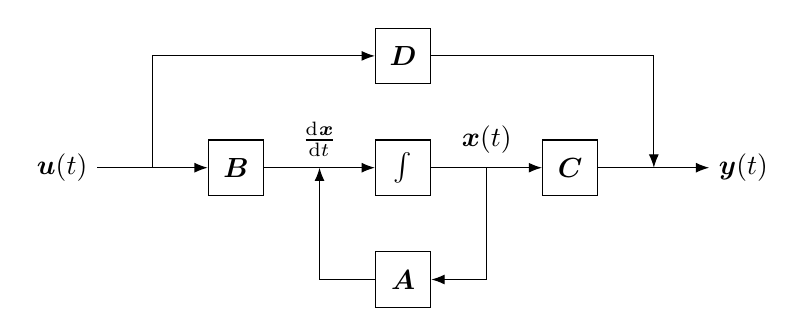
\begin{tikzpicture}[every path/.style={-Latex}, every node/.style={minimum height=20pt, minimum width=20pt}, node distance=20pt and 40pt]
    \node (u) {$\bm u(t)$};
    \node (B) [draw, right=of u] {$\bm B$};
    \node (int) [draw, right=of B] {$\int$};
    \node (C) [draw, right=of int] {$\bm C$};
    \node (y) [right=of C] {$\bm y(t)$};
    \node (D) [draw, above=of int] {$\bm D$};
    \node (A) [draw, below=of int] {$\bm A$};

    \draw (u) -- (B) coordinate[midway](uB);
    \draw (B) -- node[above] {$\od{\bm x}{t}$} (int) coordinate[midway](Bint);
    \draw (int) -- node[above] {$\bm x(t)$} (C) coordinate[midway](intC);
    \draw (C) -- (y) coordinate[midway](Cy);
    \draw (uB) |- (D);
    \draw (D) -| (Cy);
    \draw (intC) |- (A);
    \draw (A) -| (Bint);
\end{tikzpicture}
\end{document}
